\subsection{Ordenamiento de arreglos}
La Tabla~\ref{tab:sorting} compara todas las clases de entrada para $n=10^7$.
Las figuras y los CSV permiten revisar también los tamaños menores.
TO significa que ninguna de las tres muestras terminó dentro del límite.

\begin{table}[H]
\centering\small
\begin{tabular}{llrrrr}
\hline
Entrada & Dominio & Merge & Quick & Patience & \texttt{std::sort}\\
\hline
Aleatorio & D1 & 0.673 & TO & 1.712 & 0.187 \\
Aleatorio & D7 & 1.240 & 0.742 & 4.309 & 0.653 \\
Ascendente & D1 & 0.464 & TO & 1.484 & 0.083 \\
Ascendente & D7 & 0.457 & 0.175 & 15.979$^{*}$ & 0.119 \\
Descendente & D1 & 0.478 & TO & 0.681 & 0.084 \\
Descendente & D7 & 0.498 & 0.236 & 0.666 & 0.107 \\
\hline
\end{tabular}
\caption{Tiempo medio en segundos para $n=10^7$. $^{*}$PatienceSort ascendente
D7: una muestra completada y dos timeouts; no es una media de tres éxitos.}
\label{tab:sorting}
\end{table}

\subsubsection{MergeSort}
MergeSort divide el arreglo en mitades y después mezcla las partes ordenadas
\cite{geeksforgeeks_mergesort}. La división tiene aproximadamente $\log_2 n$
niveles; en cada nivel de mezcla se procesa una cantidad total de elementos
proporcional a $n$. Esto explica el costo $O(n\log n)$ \cite{algorithms_erickson}.
Nuestro código crea vectores auxiliares y copia elementos en cada mezcla.
También realiza la división y la mezcla si la entrada ya está ordenada:
no incorpora una comprobación para saltarse las mezclas que no hagan falta.

Para $n=10^7$, los promedios fueron de 0,457 a 1,240 s según la configuración.
Las entradas aleatorias D7 fueron más lentas que las ascendentes D7
(1,240 frente a 0,457 s). Por lo tanto, compartir el mismo orden de complejidad
no implica tener el mismo tiempo para todas las entradas. Su memoria máxima
rondó los 98,7 MiB en ese tamaño, frente a unos 79,8 MiB de \texttt{std::sort}.
Los vectores auxiliares son una explicación coherente con esta diferencia,
aunque no se midió por separado el costo de cada copia.

\subsubsection{QuickSort}
La implementación usa el elemento central como pivote y una partición de
Lomuto \cite{geeksforgeeks_quicksort}. Cada partición recorre el segmento
actual. Si las divisiones están equilibradas, el costo esperado es
$O(n\log n)$; si quedan muy desbalanceadas, puede llegar a $O(n^2)$
\cite{algorithms_erickson}. Por ejemplo, con todos los valores iguales,
la condición \texttt{<=} deja casi todos los elementos al mismo lado.
El trabajo pasa a ser proporcional a $(n-1)+(n-2)+\cdots+1$.

En D1 solo existen diez valores posibles, por lo que las entradas grandes
contienen muchas repeticiones. Las nueve pruebas de $n=10^7$ en D1 terminaron
en timeout. En D7 sí terminaron las nueve, con medias de 0,742 s en aleatorio,
0,175 s en ascendente y 0,236 s en descendente. Este contraste es consistente
con el efecto de los duplicados en la partición, pero no contamos las
particiones ni demostramos experimentalmente que fueran la única causa.
Elegir un pivote central no resuelve por sí solo ese problema.

\begin{figure}[H]
\centering
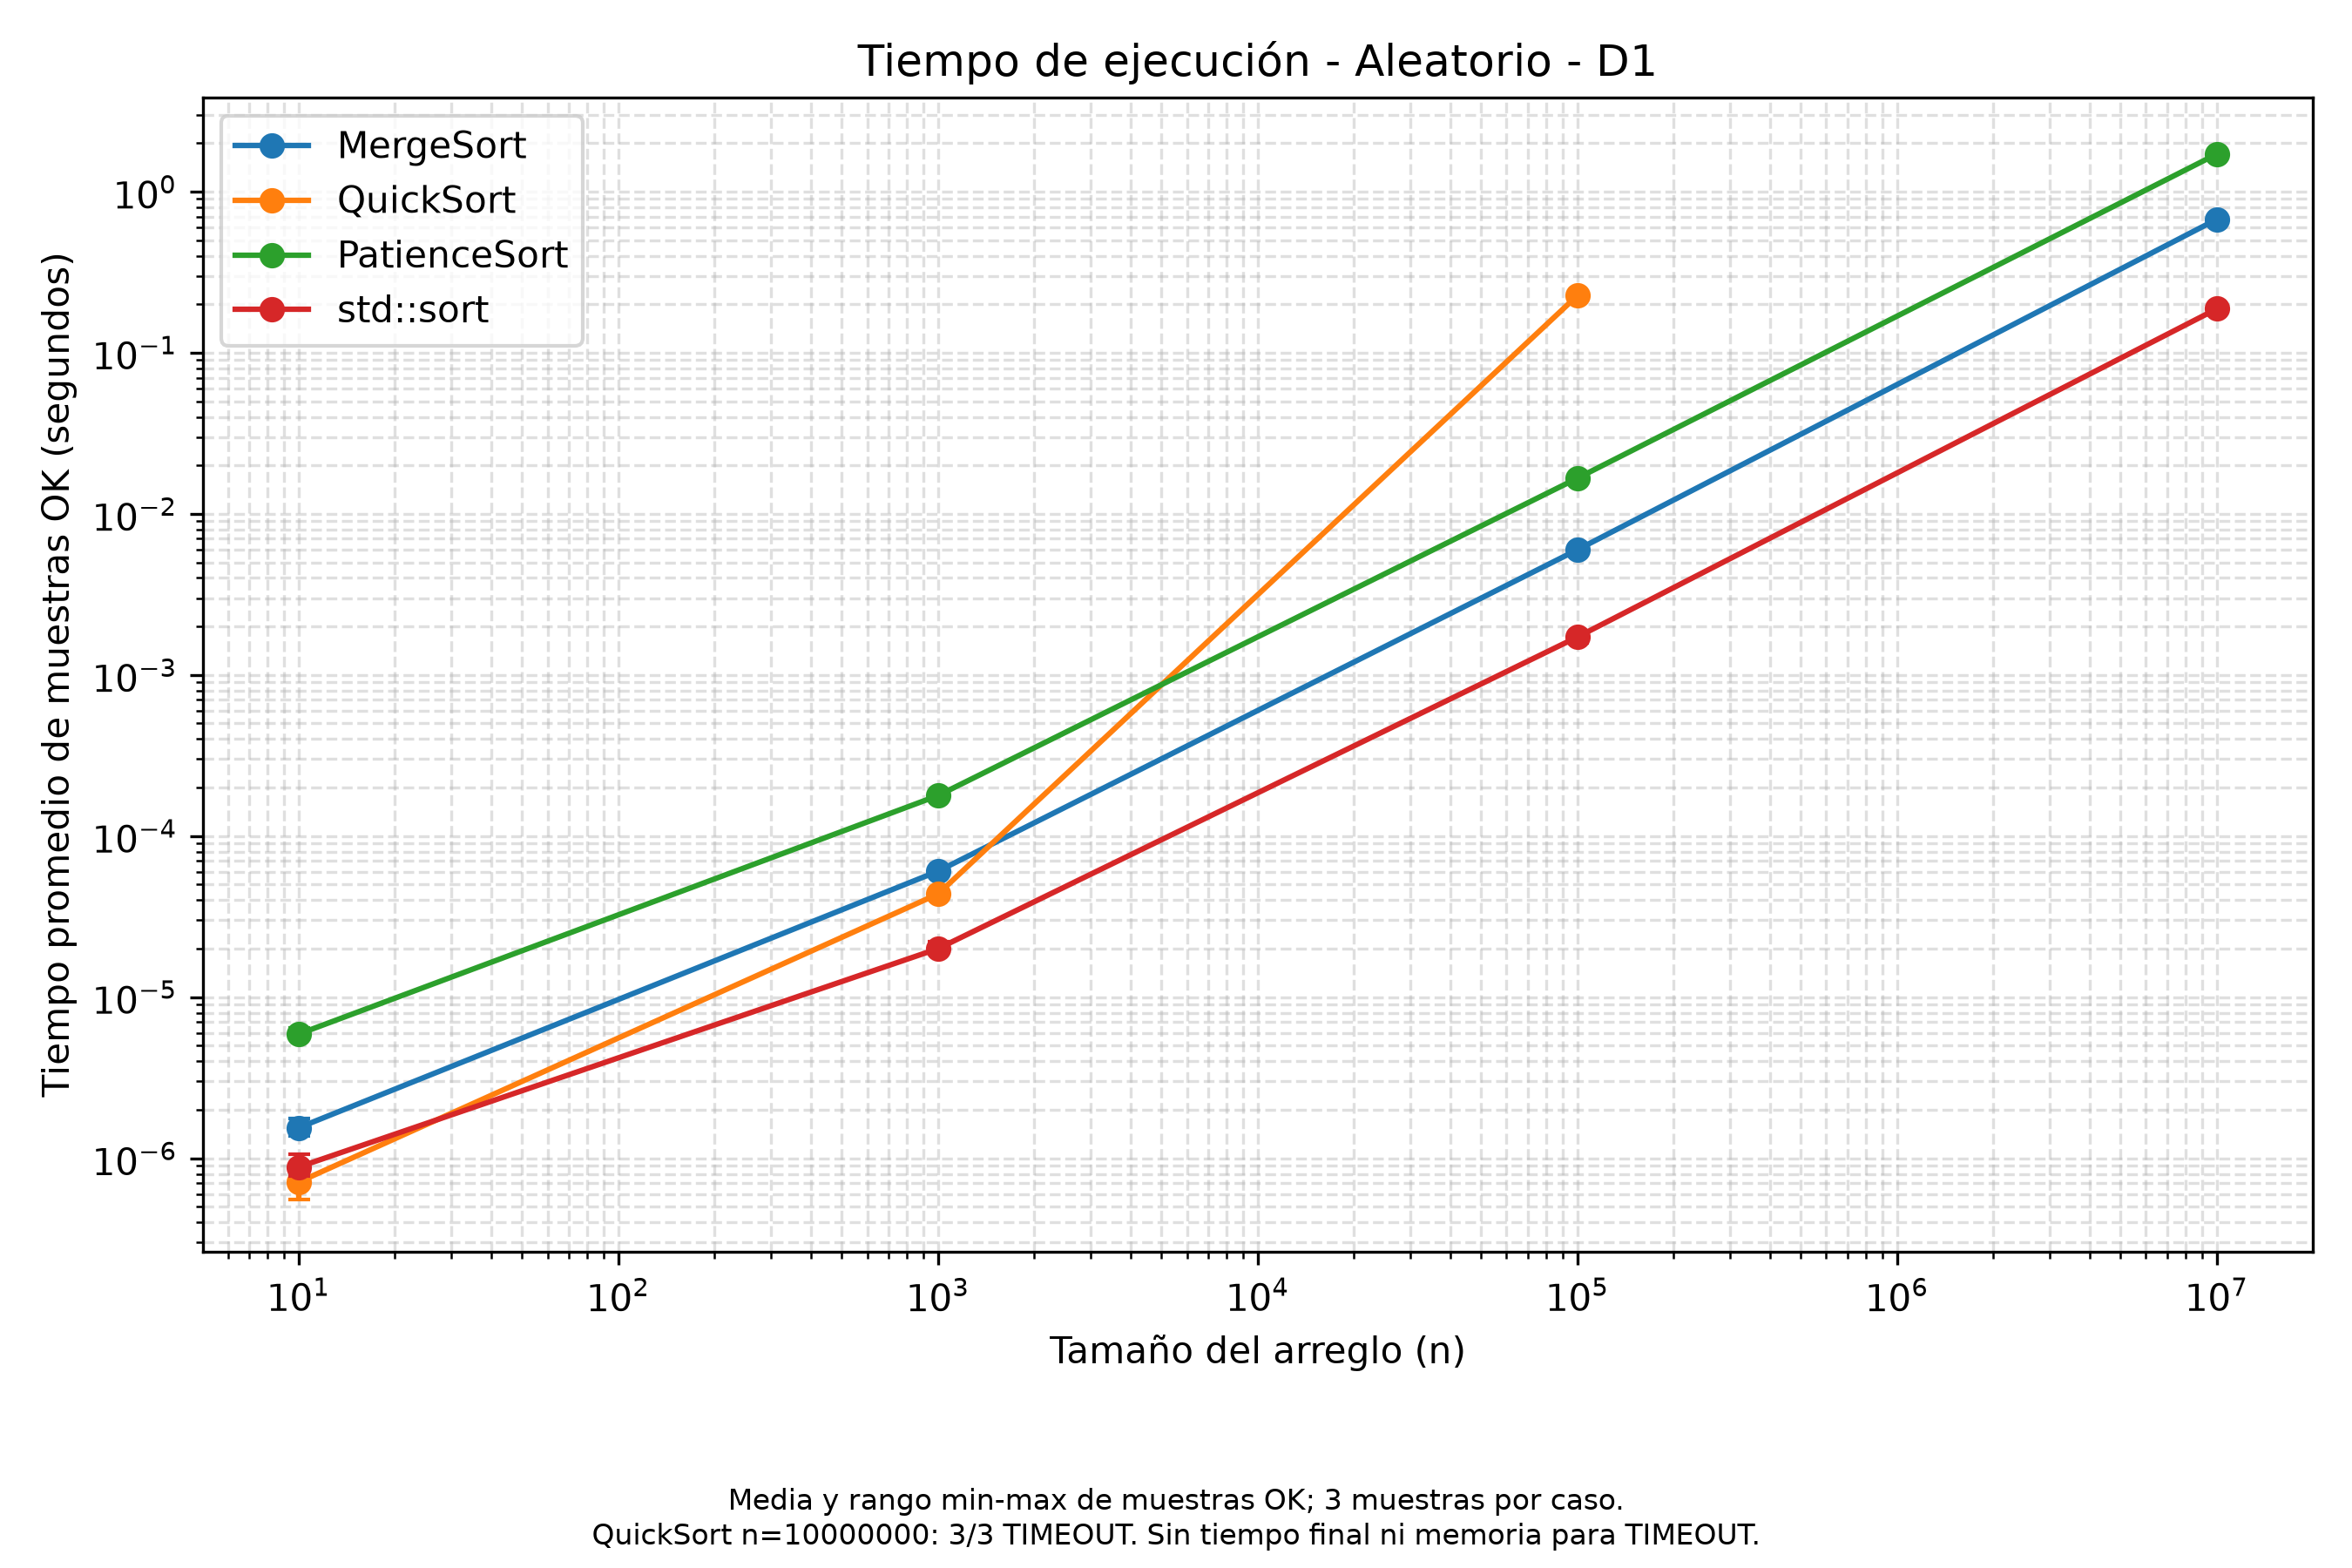
\includegraphics[width=.80\textwidth]{../code/sorting/data/plots/tiempo_aleatorio_D1.png}
\caption{Tiempo en entradas aleatorias D1. La nota identifica los tres timeouts de QuickSort en el tamaño mayor.}
\label{fig:d1}
\end{figure}

\subsubsection{PatienceSort}
PatienceSort distribuye los valores en pilas y luego los extrae mediante
un heap \cite{rosettacode_patiencesort}. Nuestro código busca la pila con
búsqueda binaria. Con $k$ pilas, esa búsqueda tiene costo $O(\log k)$;
las operaciones del heap también dependen de $k$. La organización habitual
permite un costo $O(n\log n)$, pero el número de pilas y sus estructuras
auxiliares influyen en el costo concreto de esta implementación.

En una entrada ascendente con muchos valores distintos se forman muchas pilas.
En D7 y $n=10^7$ hubo dos timeouts y una muestra completada en 15,979 s,
con 5,42 GiB de memoria máxima. En descendente D7 la media fue de 0,666 s
y aproximadamente 82,0 MiB. Es una diferencia grande para el mismo tamaño.
La cantidad de pilas y las asignaciones asociadas ofrecen una explicación
plausible, sin que hayamos medido ese costo de forma aislada. El punto de
15,979 s representa solo el caso terminado; omitir los otros dos resultados
haría parecer más favorable el comportamiento de esta configuración.

\subsubsection{\texttt{std::sort}}
Se utilizó directamente la función de la biblioteca estándar
\cite{cppreference_sort}, cuya garantía de comparaciones es $O(n\log n)$.
Para $n=10^7$ tuvo la menor media entre las ejecuciones completadas en las
seis configuraciones: de 0,083 a 0,653 s. En aleatorio D1 fue de 0,187 s,
frente a 0,673 s de MergeSort y 1,712 s de PatienceSort. En aleatorio D7
la distancia con QuickSort fue menor: 0,653 frente a 0,742 s.

Estos resultados muestran que la notación asintótica no distingue todos los
costos de una implementación. No medimos el número de operaciones internas
de \texttt{std::sort}, por lo que no atribuimos su ventaja a una única
optimización. Tampoco generalizamos el orden observado a otros equipos o
bibliotecas. En los tamaños mínimos, los tiempos son muy pequeños y una
única ejecución por muestra no basta para interpretar diferencias pequeñas.

\begin{figure}[H]
\centering
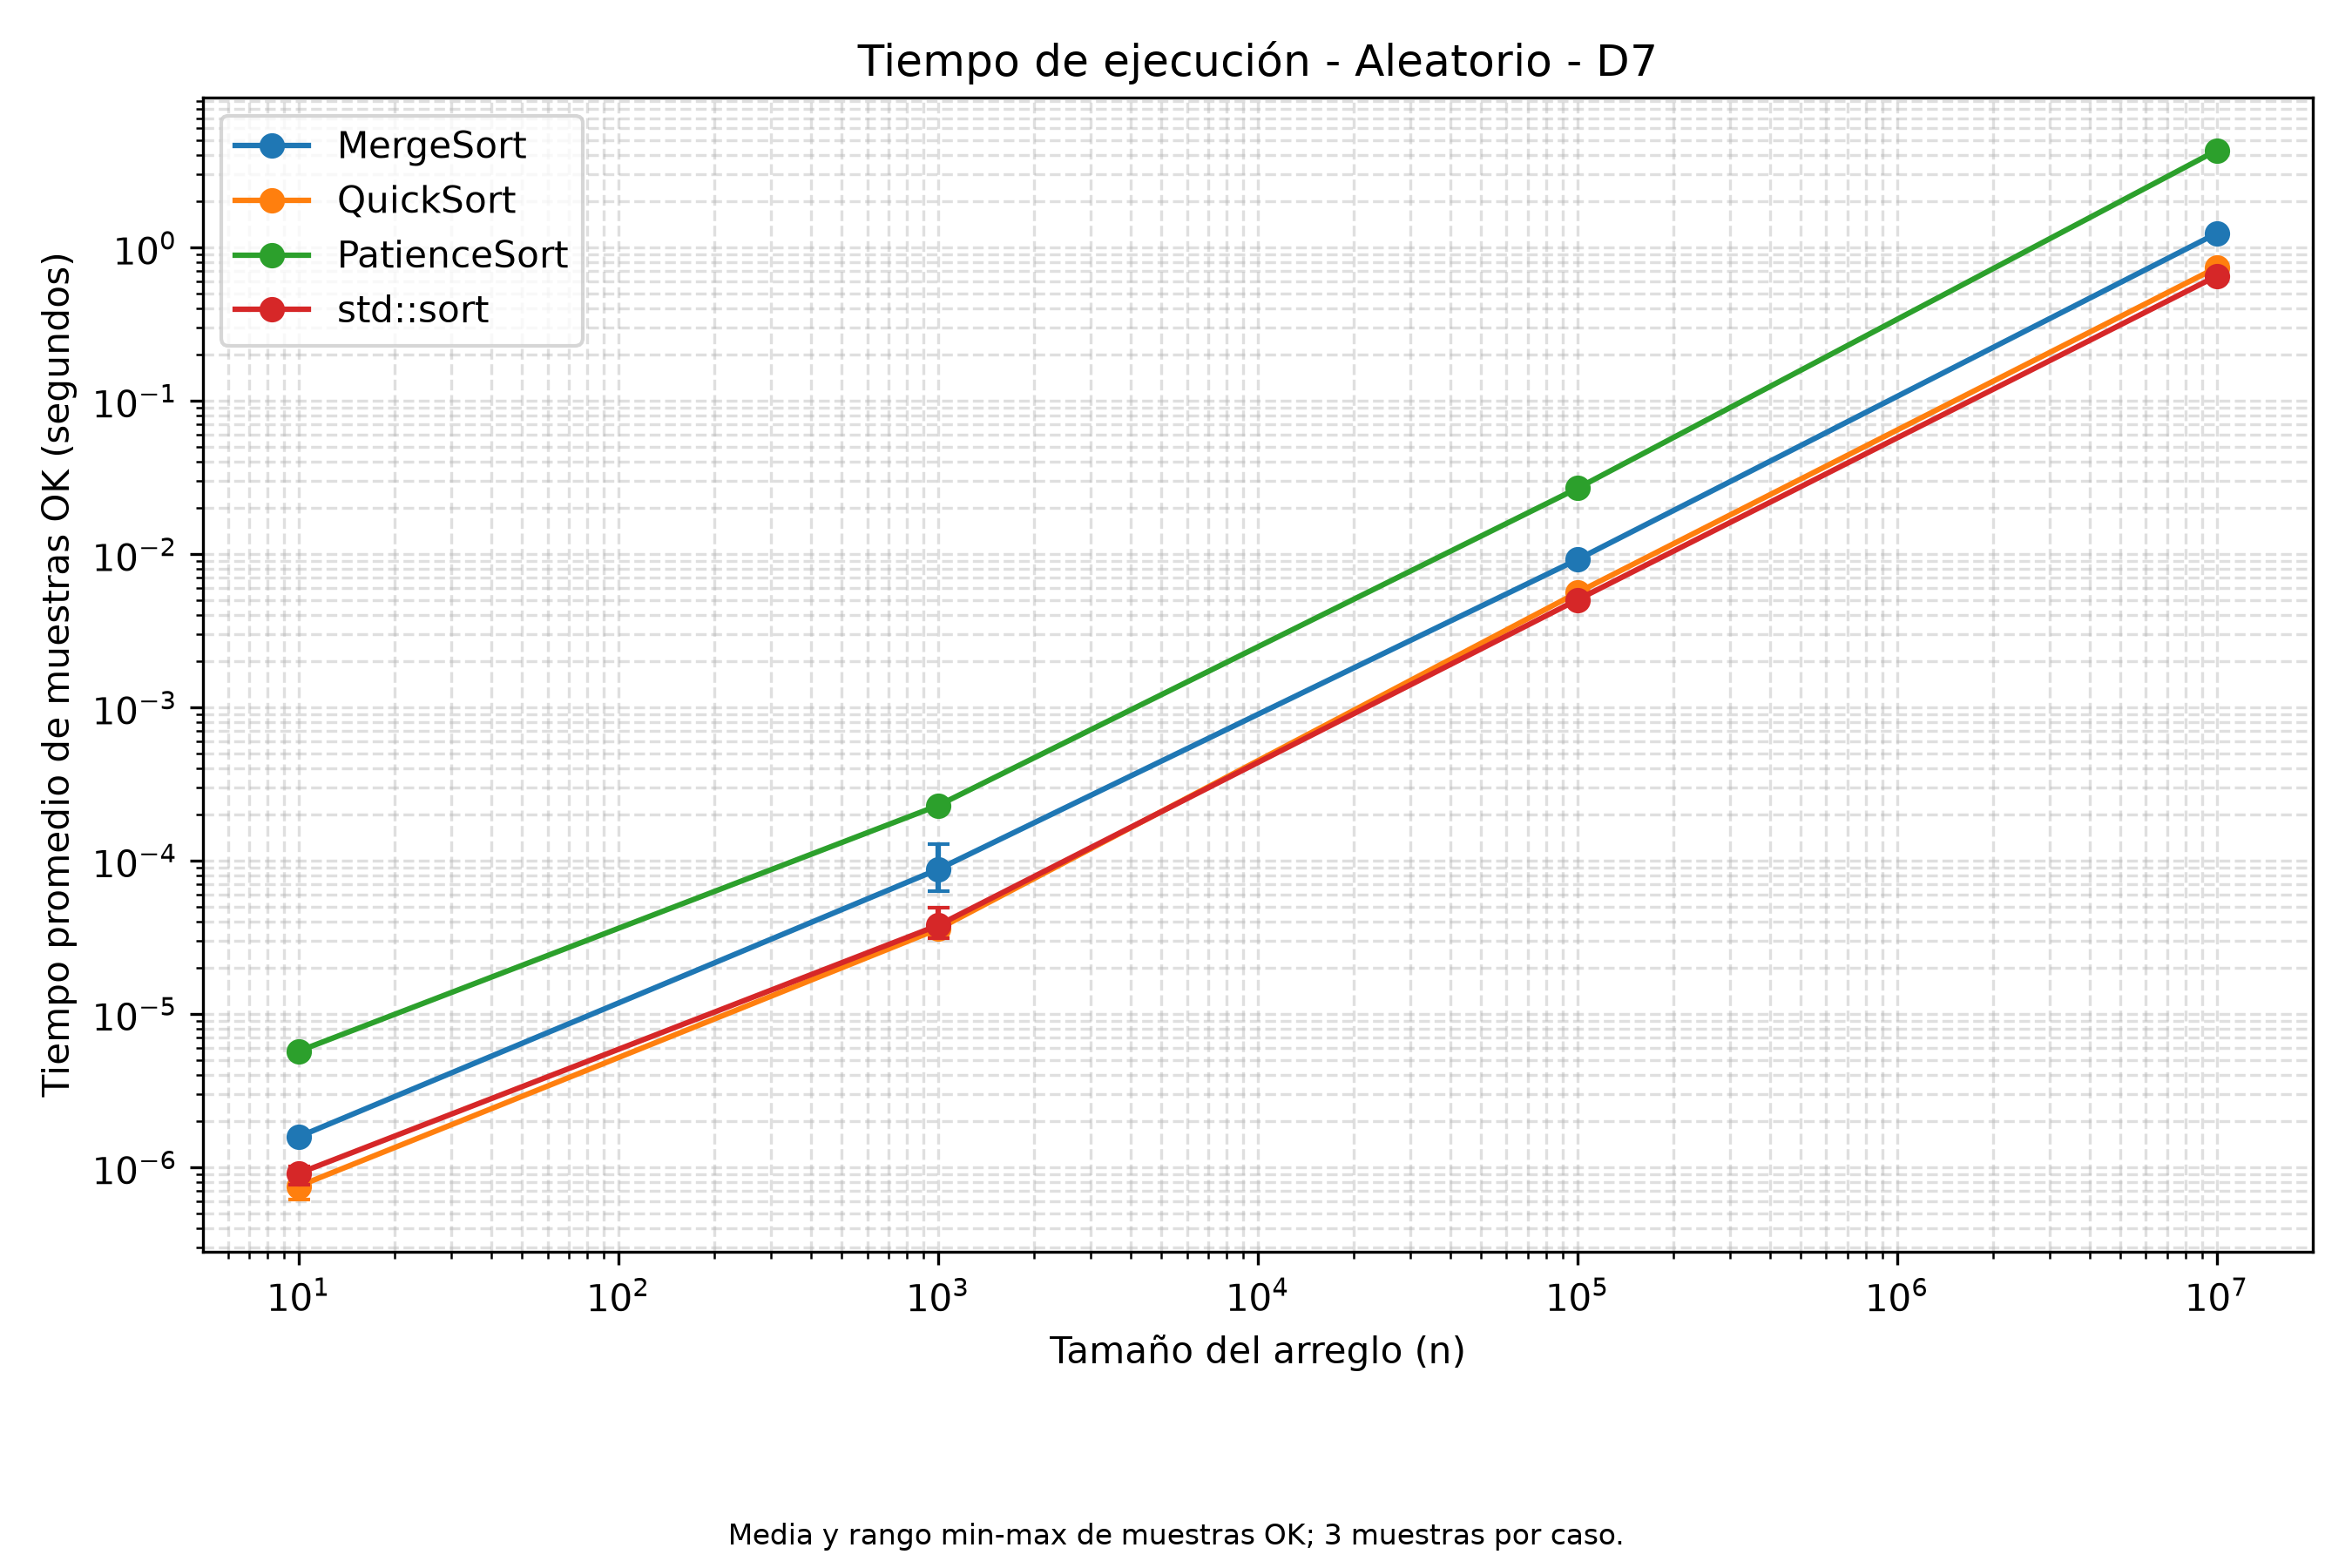
\includegraphics[width=.80\textwidth]{../code/sorting/data/plots/tiempo_aleatorio_D7.png}
\caption{Tiempo en entradas aleatorias D7. Las barras muestran el rango de las tres muestras, no intervalos de confianza.}
\label{fig:d7}
\end{figure}

\begin{figure}[H]
\centering
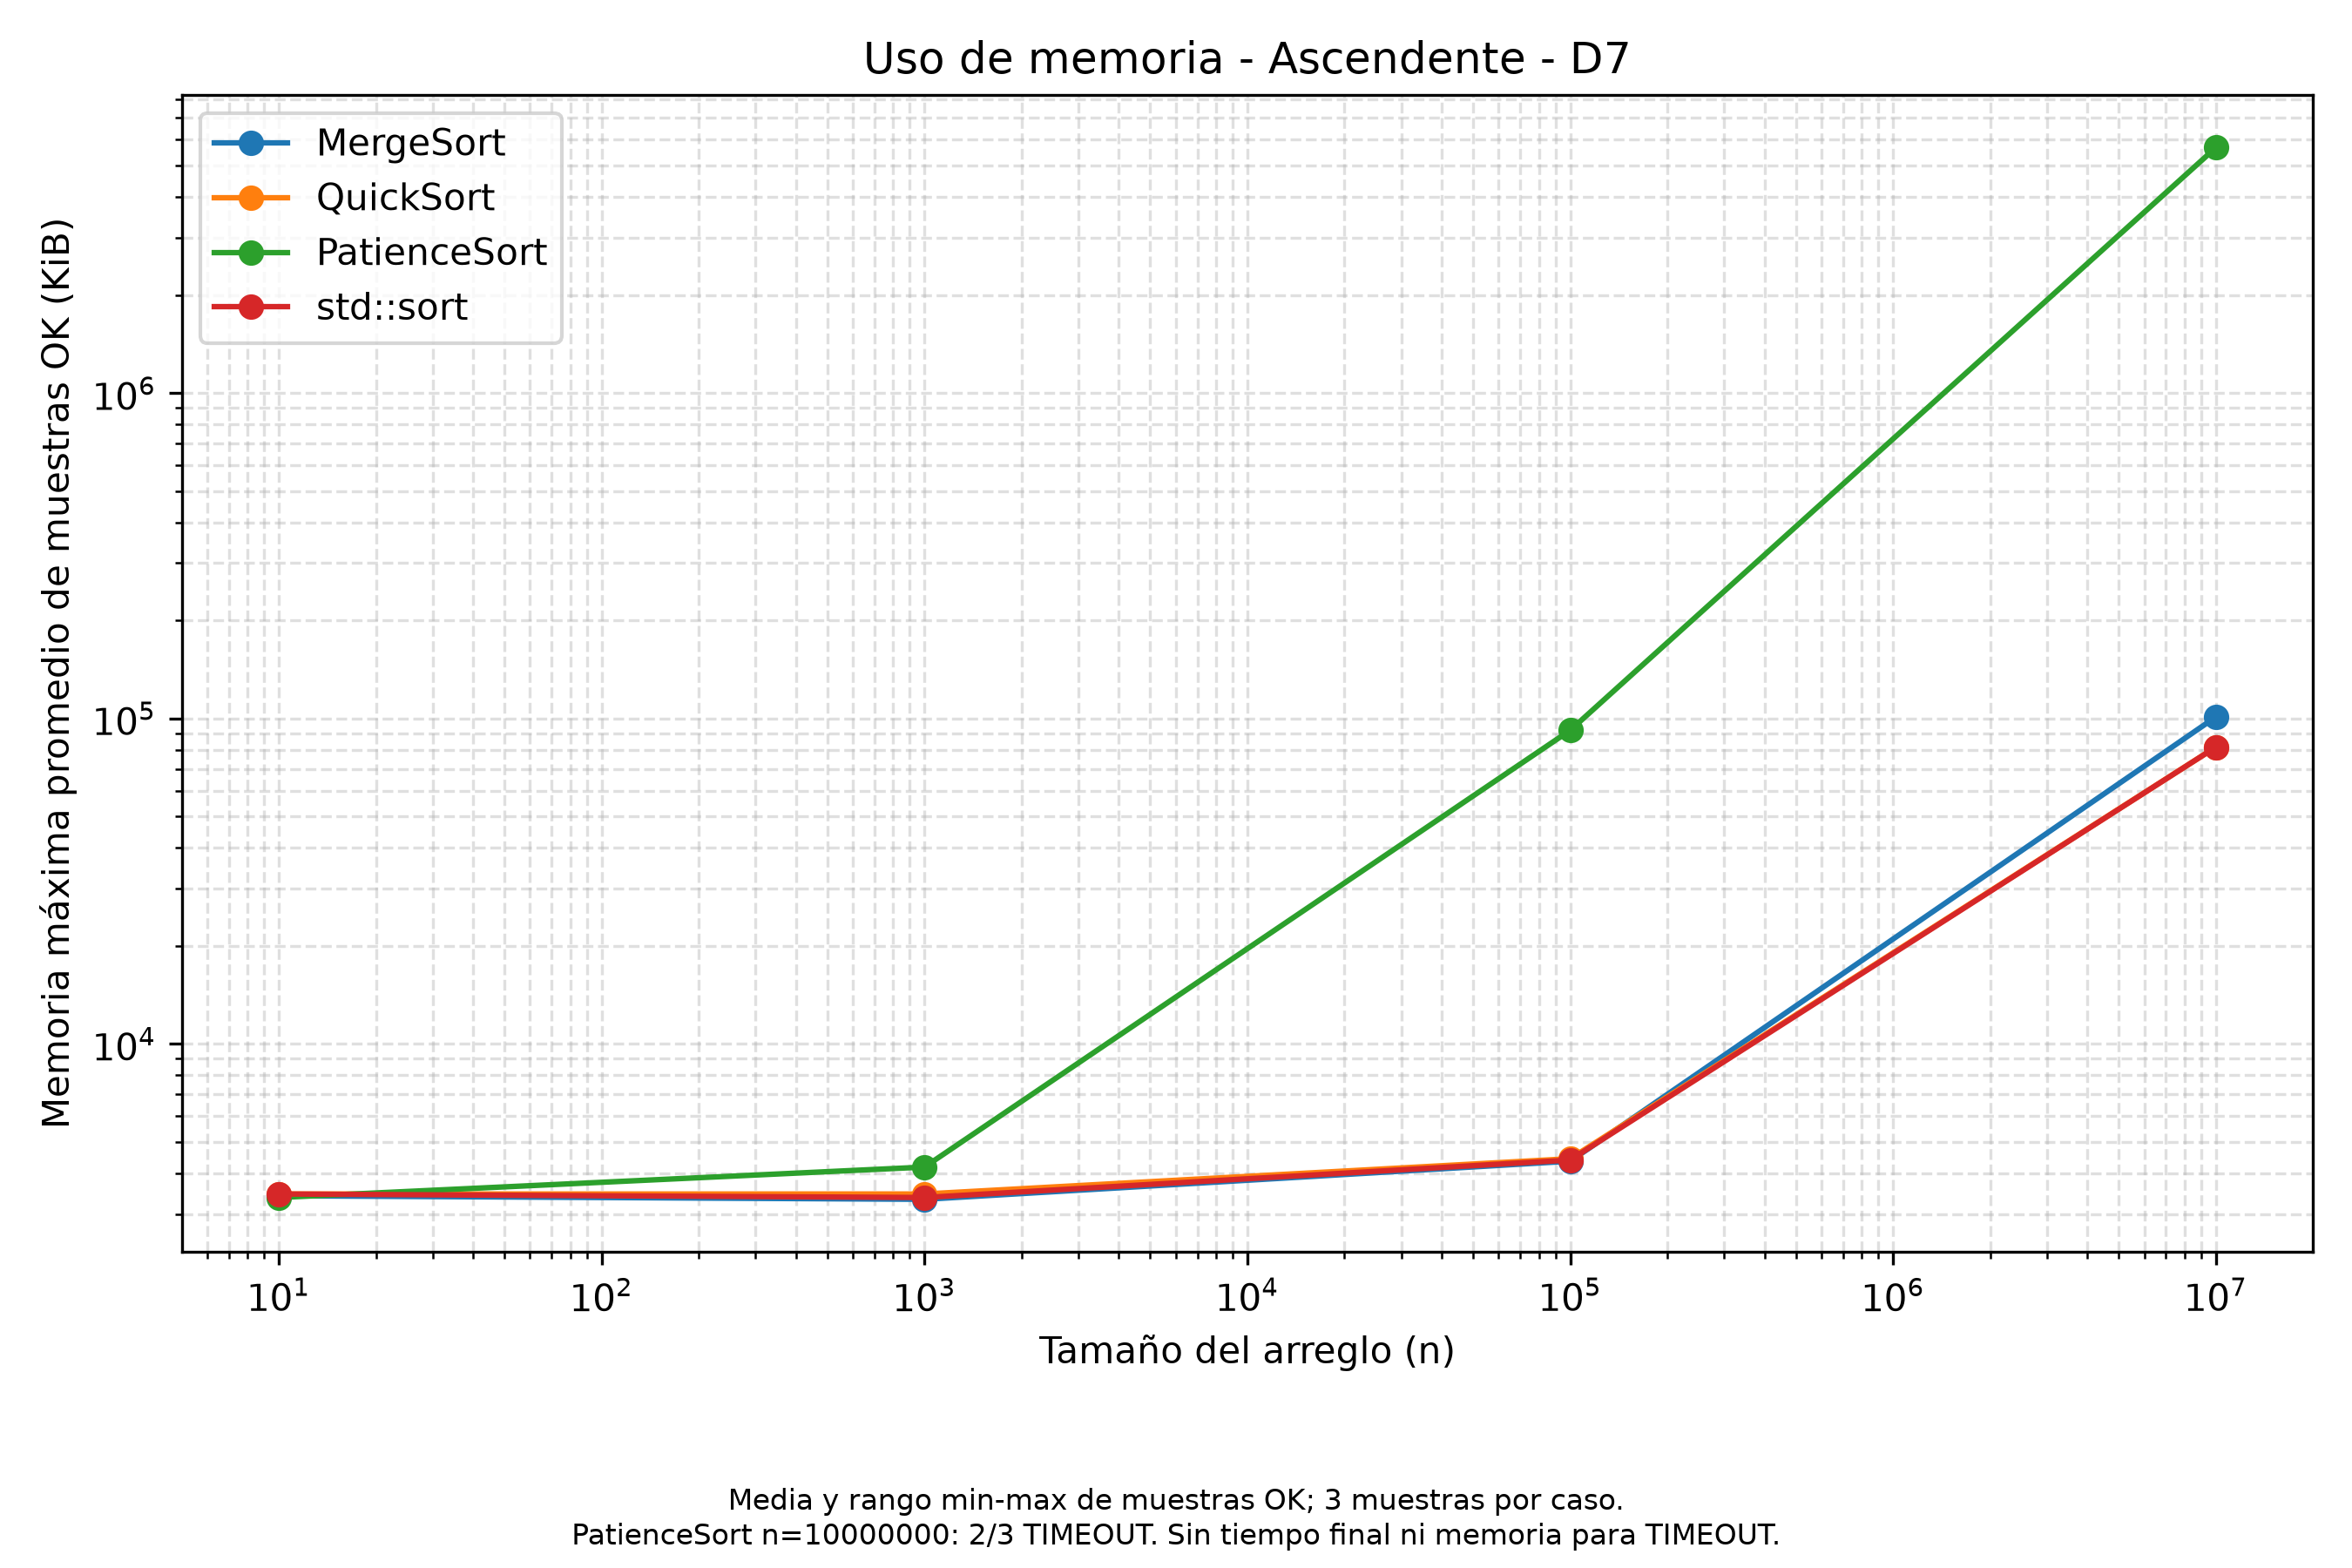
\includegraphics[width=.80\textwidth]{../code/sorting/data/plots/memoria_ascendente_D7.png}
\caption{Memoria máxima del proceso en ascendente D7, con ambos ejes logarítmicos. El dato grande de PatienceSort corresponde solo a una muestra completada.}
\label{fig:sortmemory}
\end{figure}

\subsection{Multiplicación de matrices}
\subsubsection{Naive}
Naive calcula cada una de las $n^2$ posiciones del resultado con un recorrido
de longitud $n$: realiza $n^3$ multiplicaciones escalares
\cite{geeksforgeeks_naive}. Los tres ciclos se ejecutan también sobre los
ceros; el código no aprovecha de forma especial las matrices diagonales
ni las dispersas. Por eso, tener menos valores no nulos no elimina esos
recorridos ni convierte esta implementación en un algoritmo para matrices dispersas.

\begin{table}[H]
\centering\small
\begin{tabular}{rrr}
\hline
$n$ & Naive (s) & Strassen (s)\\
\hline
16 & \num{3.972e-06} & \num{0.00107331} \\
64 & \num{0.000117777} & \num{0.0493432} \\
256 & \num{0.00650711} & \num{2.35752} \\
1024 & \num{1.12541} & TO (3/3) \\
\hline
\end{tabular}
\caption{Tiempo medio para matrices diagonales D0. Los valores se calcularon
con los CSV de la corrida final. TO indica timeout, no un tiempo medido.}
\label{tab:matrix}
\end{table}

\subsubsection{Strassen}
Strassen usa siete multiplicaciones recursivas de submatrices en lugar de ocho,
a cambio de sumas y restas adicionales \cite{geeksforgeeks_strassen}.
La recurrencia $T(n)=7T(n/2)+O(n^2)$ da un costo
$O(n^{\log_2 7})\approx O(n^{2,807})$, mejor asintóticamente que el costo
cúbico de Naive \cite{algorithms_erickson}. Esto describe el crecimiento,
pero no garantiza un menor tiempo para cualquier tamaño.

Nuestra implementación copia matrices, construye submatrices y realiza
operaciones auxiliares en cada nivel. Además, llega hasta matrices de
$1\times1$, sin cambiar a Naive para los casos pequeños. Esos costos son
una explicación consistente con el resultado observado: Strassen fue más
lento en todas las configuraciones donde ambos terminaron y alcanzó el límite
en las 18 pruebas de $n=1024$. No se midió por separado cuánto corresponde
a copias, recursión o asignaciones, ni se encontró un tamaño de cruce donde
Strassen gane. Usar Naive como caso base sería un experimento futuro, no
una mejora evaluada en esta entrega.

\begin{figure}[H]
\centering
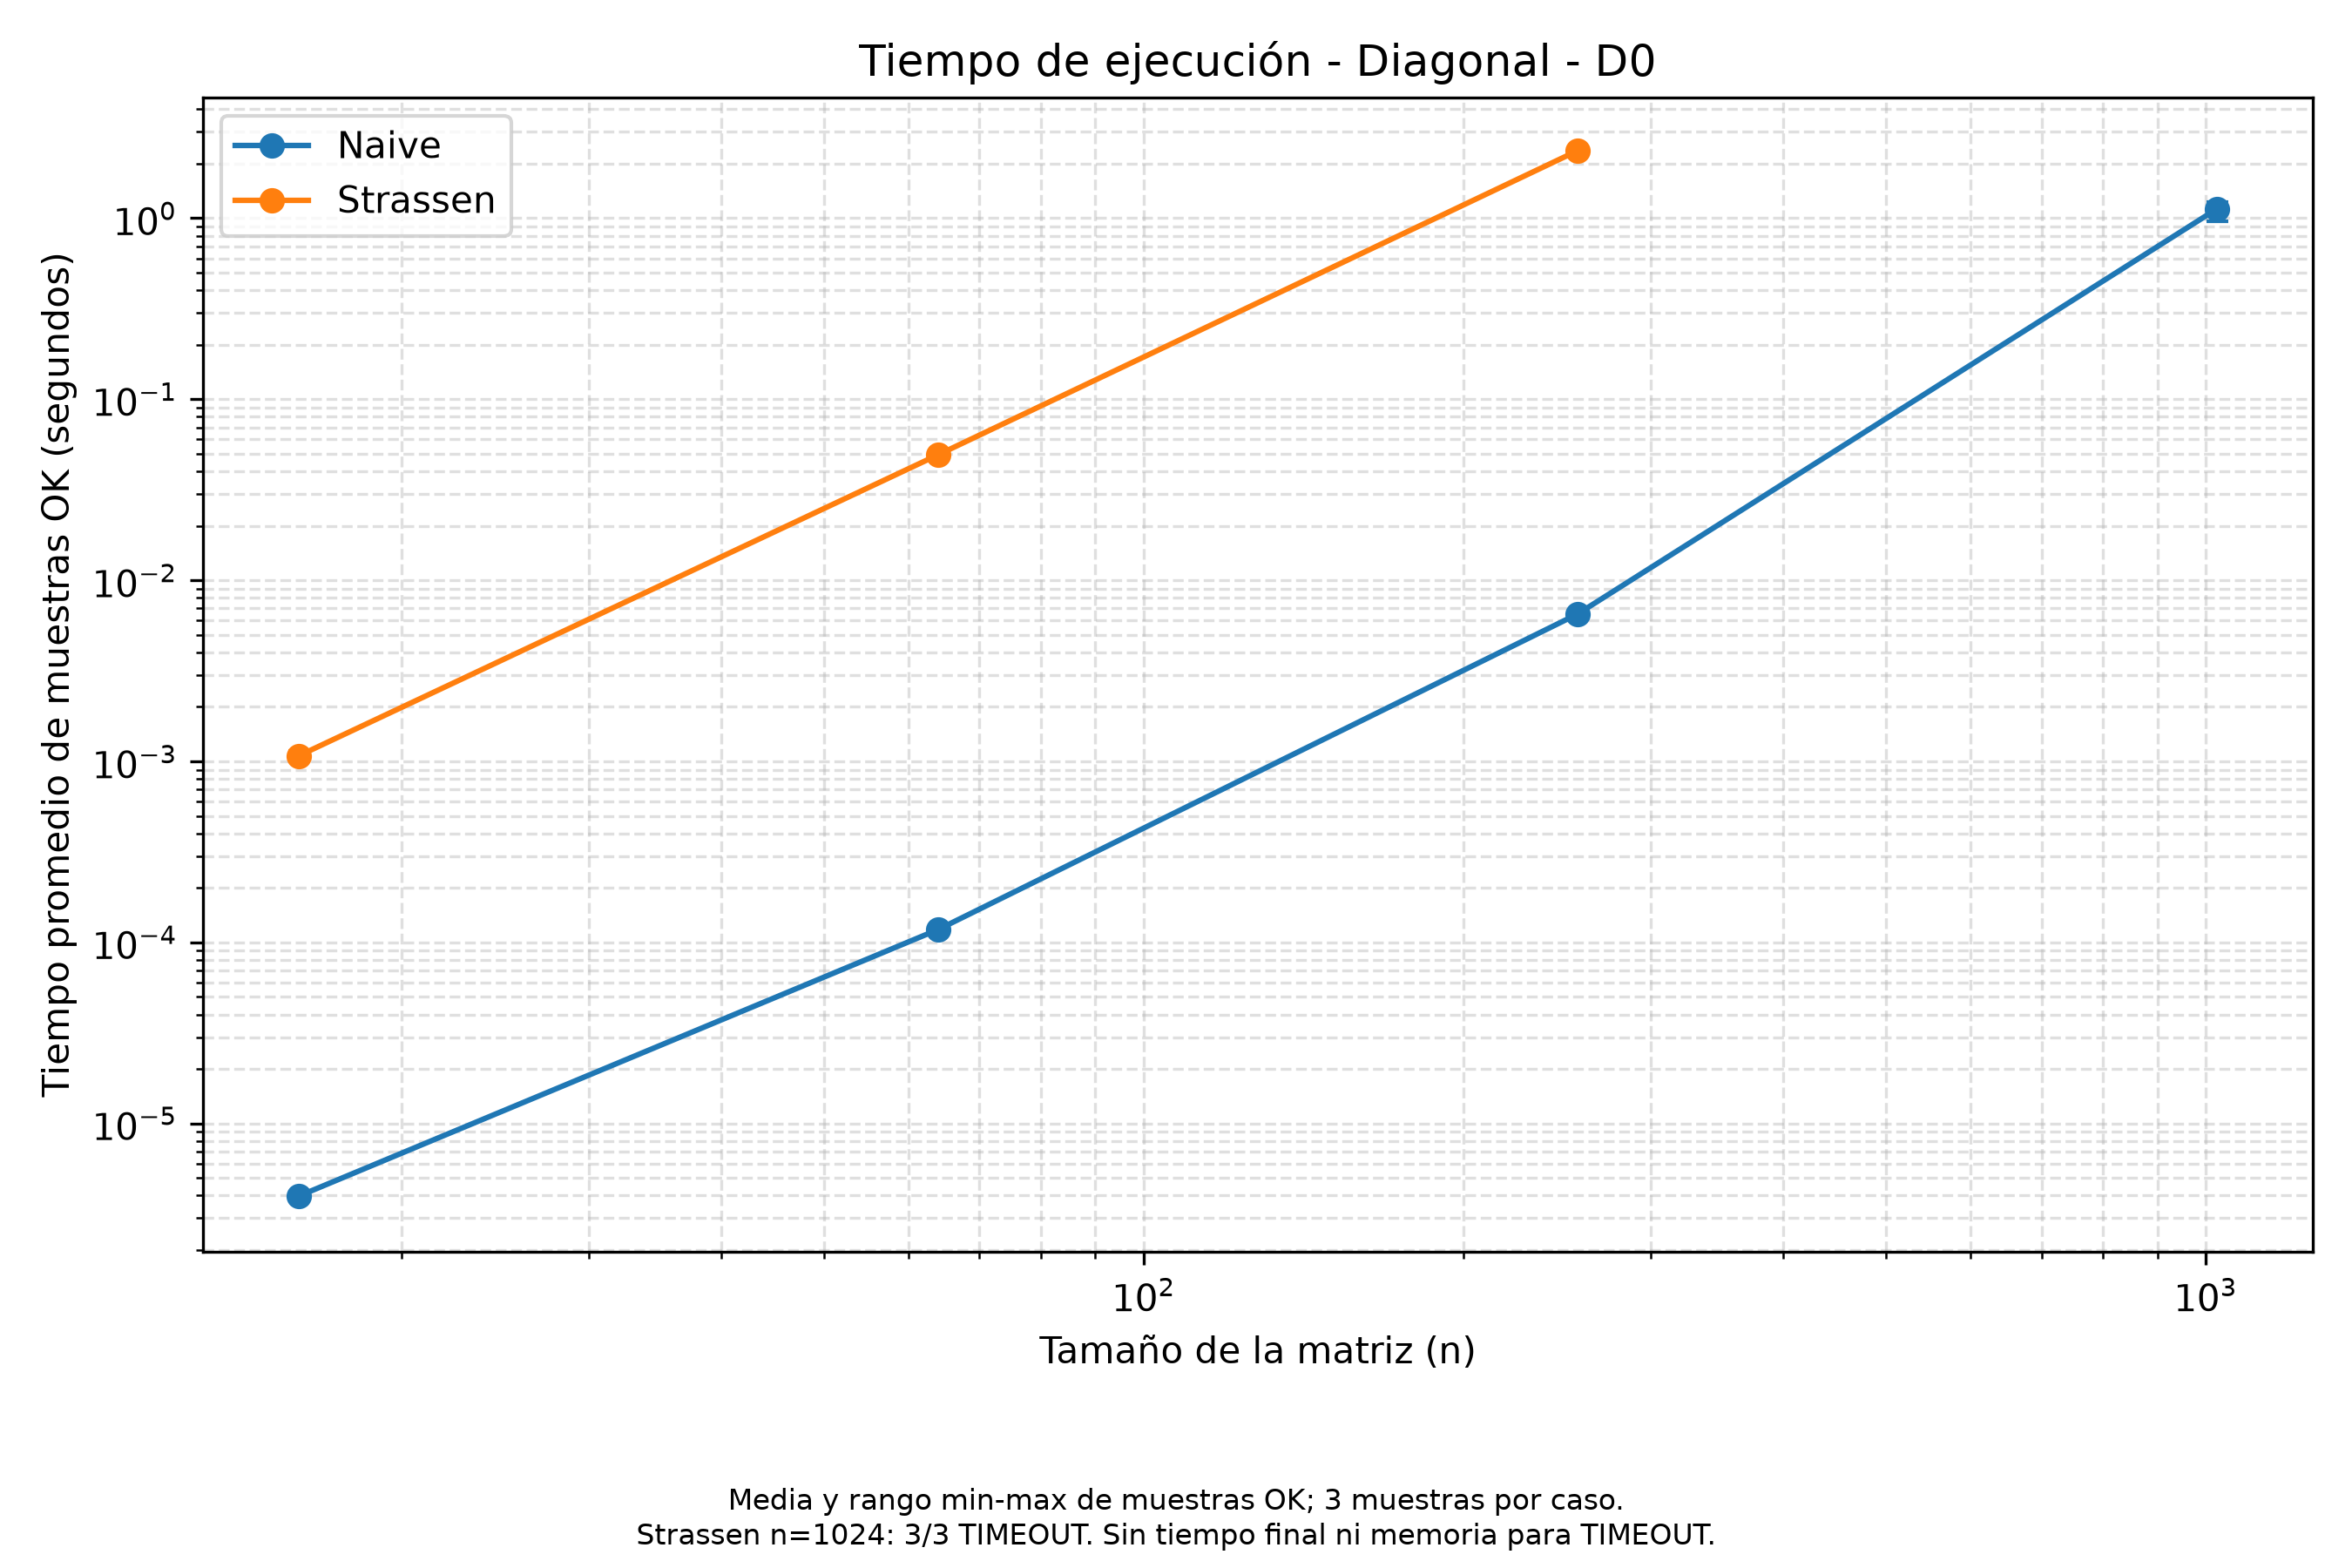
\includegraphics[width=.80\textwidth]{../code/matrix_multiplication/data/plots/tiempo_matriz_diagonal_D0.png}
\caption{Tiempo de matrices diagonales D0. Strassen no tiene un tiempo final registrado en 1024; las tres muestras llegaron al límite del proceso de 60 s.}
\label{fig:matrix}
\end{figure}

\subsubsection{Comparación entre entradas y memoria}
\begin{table}[H]
\centering\small
\begin{tabular}{llrr}
\hline
Tipo & Dominio & Media Naive (s) & Rango Naive (s)\\
\hline
Densa & D0 & 0.894 & 0.891--0.899 \\
Densa & D10 & 0.909 & 0.897--0.930 \\
Diagonal & D0 & 1.125 & 0.958--1.226 \\
Diagonal & D10 & 0.903 & 0.892--0.918 \\
Dispersa & D0 & 0.880 & 0.872--0.889 \\
Dispersa & D10 & 0.903 & 0.883--0.942 \\
\hline
\end{tabular}
\caption{Naive en $n=1024$: media y rango de tres muestras por configuración.
Strassen tuvo tres timeouts en cada fila.}
\label{tab:types}
\end{table}

La Tabla~\ref{tab:types} evita concluir que los tipos de entrada sean idénticos
en tiempo. La media de diagonal D0 fue mayor que las otras, pero las tres
muestras no permiten separar el efecto de la entrada de la variación del sistema.
El hecho comprobable en el código es que los ciclos de Naive no omiten ceros.

Naive usó en promedio \num{4096} KiB en matrices dispersas D10 de tamaño 256. Strassen usó en promedio \num{7552} KiB en matrices dispersas D10 de tamaño 256. La diferencia es coherente con las matrices auxiliares de Strassen.
La medida incluye el proceso completo y no permite atribuir toda la diferencia
a una estructura concreta. En los casos de timeout no se registró memoria;
por lo tanto, no se puede comparar su consumo final con el de Naive.

\begin{figure}[H]
\centering
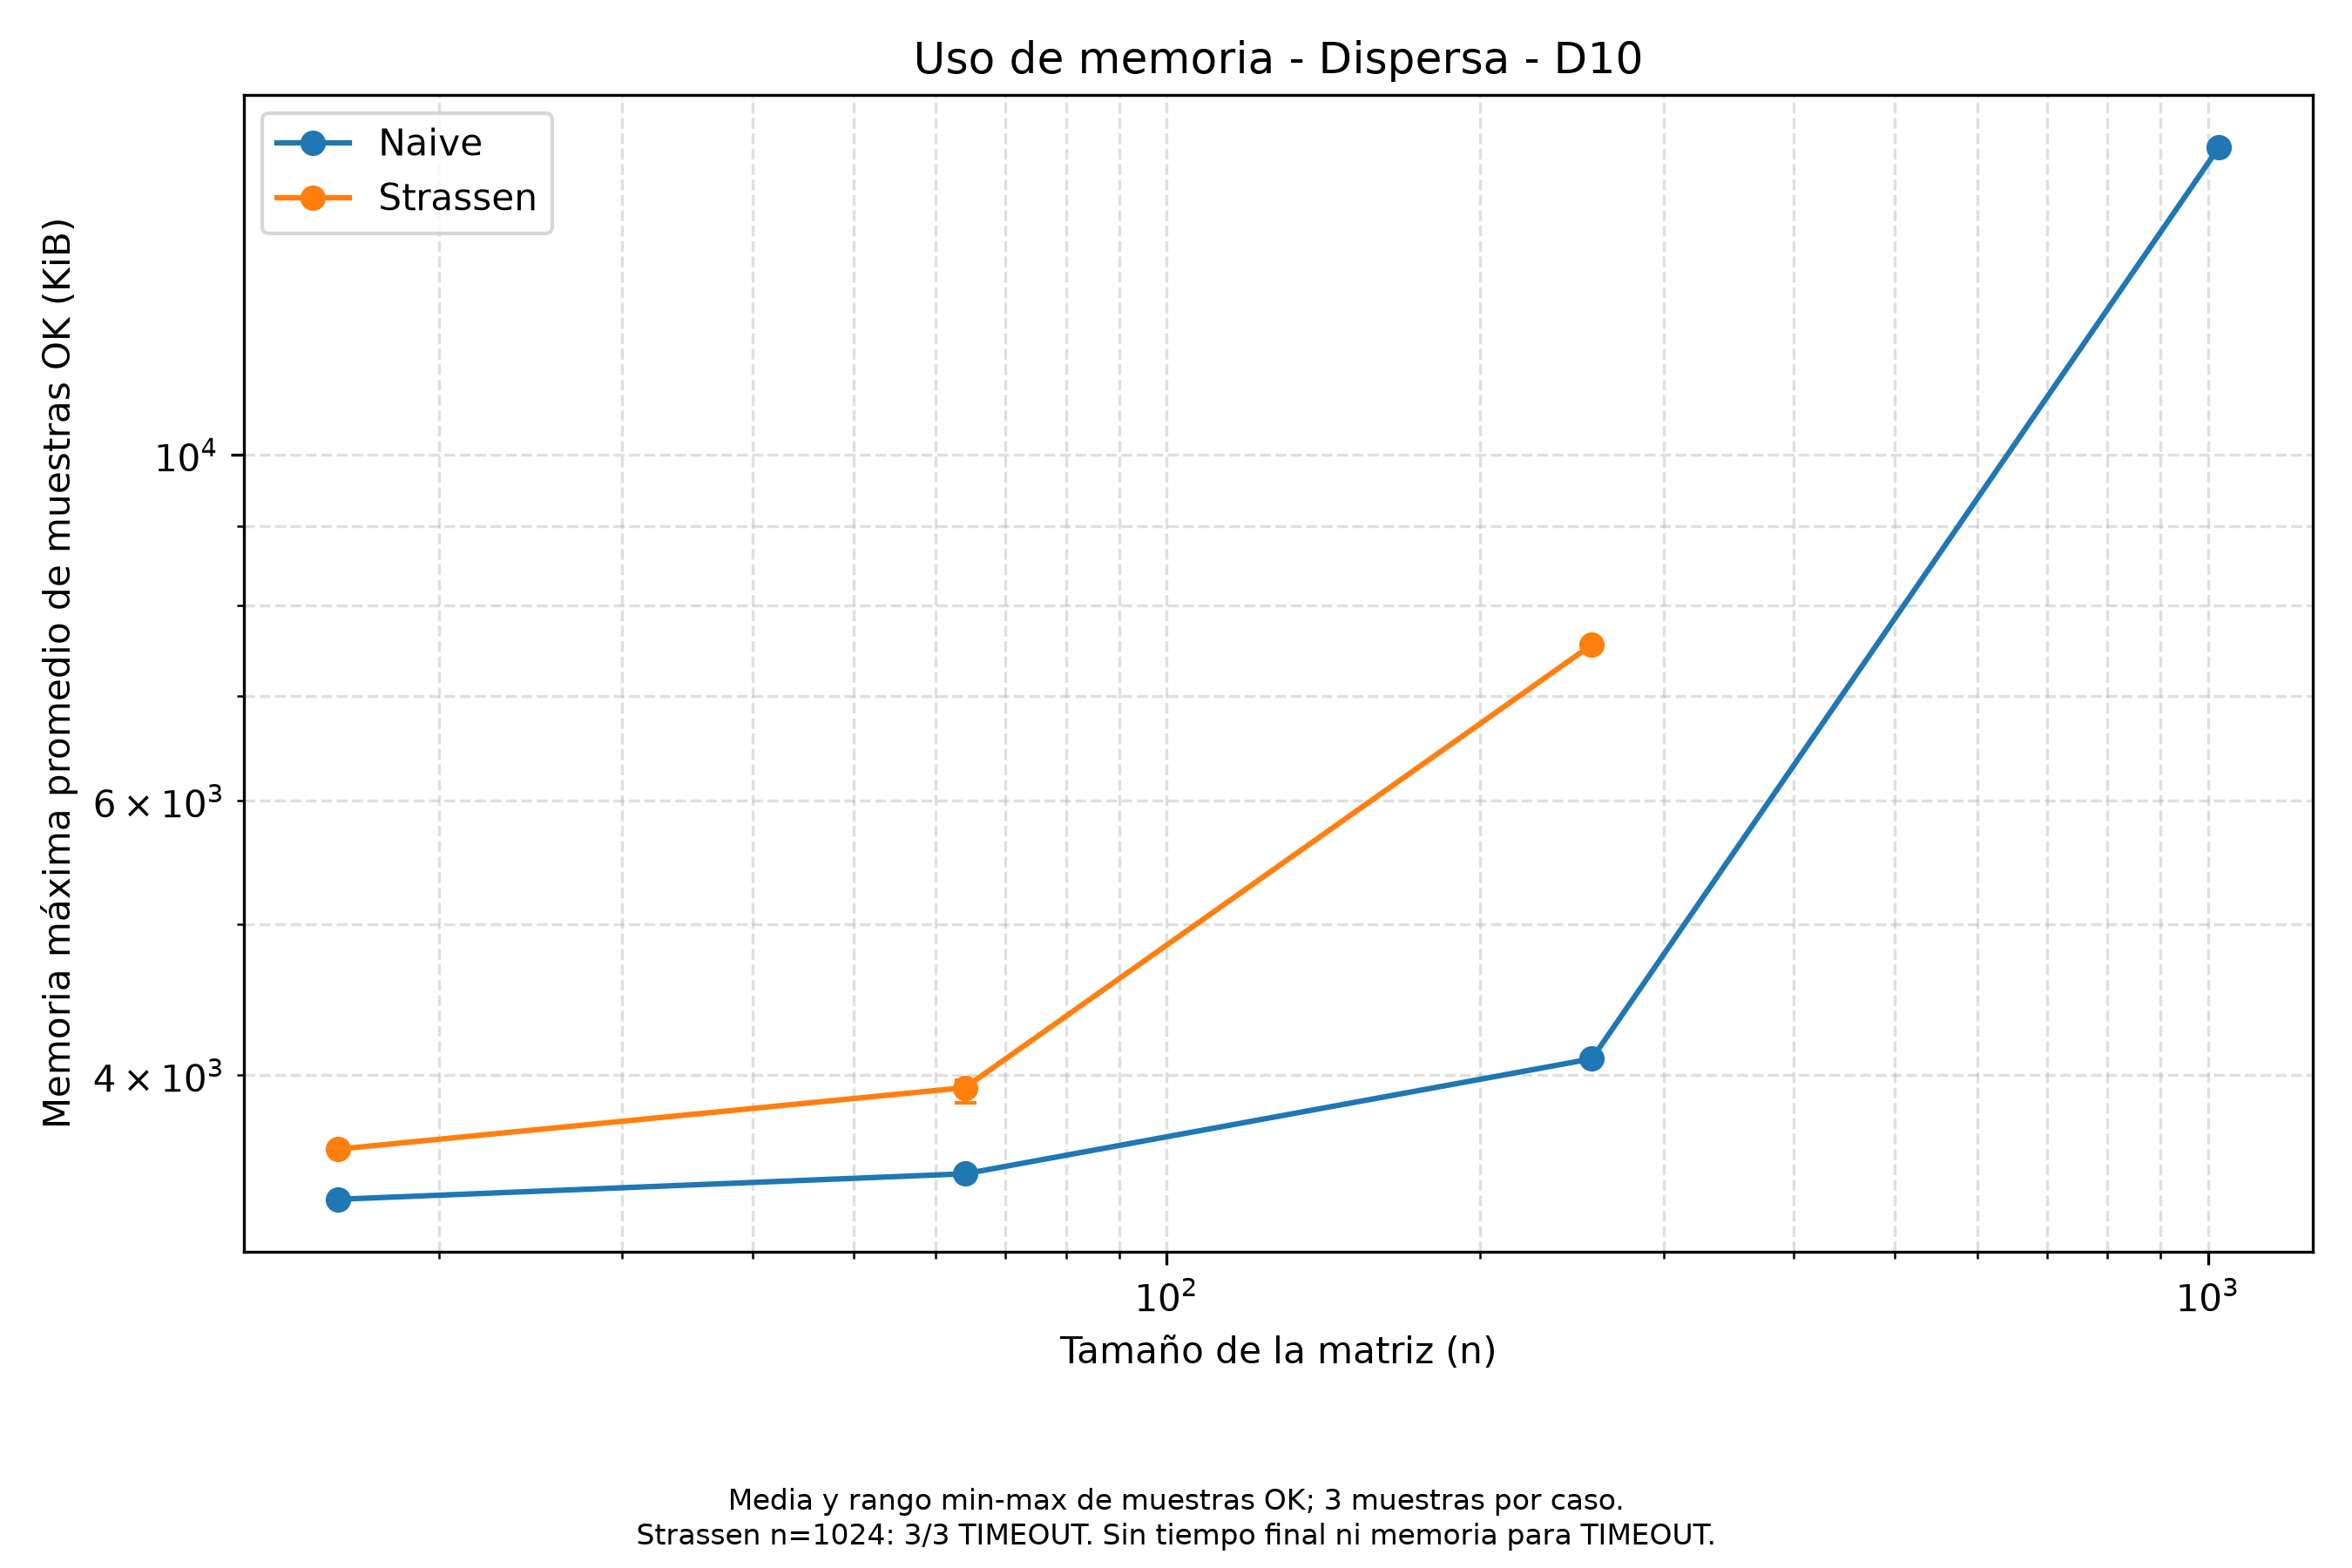
\includegraphics[width=.80\textwidth]{../code/matrix_multiplication/data/plots/memoria_matriz_dispersa_D10.png}
\caption{Memoria máxima del proceso en matrices dispersas D10. La serie de Strassen no incluye 1024 porque las ejecuciones terminaron en timeout.}
\label{fig:matrixmemory}
\end{figure}
